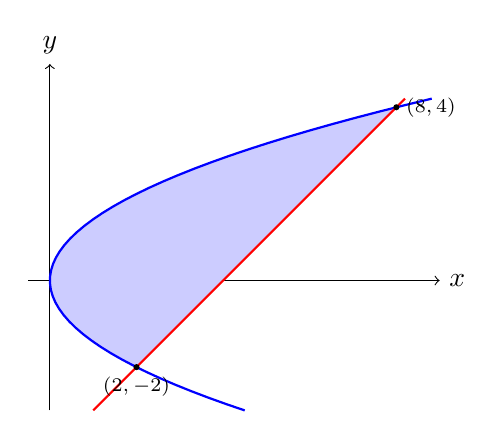
\begin{tikzpicture}[scale=0.55]
      \draw[->] (-0.5,0)--(9,0) node[right]{$x$};
      \draw[->] (0,-3)--(0,5) node[above]{$y$};
      \fill[blue!20] plot[domain=-2:4,samples=40]({\x*\x/2},{\x})
        -- plot[domain=4:-2,samples=2]({\x+4},{\x}) -- cycle;
      \draw[thick,blue] plot[domain=-3:4.2,samples=50]({\x*\x/2},{\x});
      \draw[thick,red] (1,-3)--(8.2,4.2);
      \fill (2,-2) circle (2pt) (8,4) circle (2pt);
      \node[font=\scriptsize,below] at (2,-2) {$(2,-2)$};
      \node[font=\scriptsize,right] at (8,4) {$(8,4)$};
    \end{tikzpicture}